% Drawing 142/03-4 -- folder 142, batch 03, archive page 57 (PDF page 58).
% Transcription: en marge, un petit schéma : $P_\varepsilon$ relié par un lacet $l_0$ au trou $R_{\omega i} \simeq R_0$ (d'orientation $\varpi = \omega \wedge \varepsilon$), au point $Q_\infty$ et au trou $R_{\omega' i} \simeq R_1$.
% Kind: small loop diagram between holes. Method 2 (schematic redraw from the facsimile). Status: partial.
% Notes: P_epsilon at the left; the hole R_{omega i} = R_0 at the top right (circle) and the hole R_{omega' i} at the bottom (circle); Q_infty between them. The strokes as on the page: a double stem from P_epsilon to the top circle (the return stroke arrowed towards P_epsilon); from the point B on the lower left of the top circle a stroke down through Q_infty that crosses the next stroke and ends, arrowed, inside the bottom circle; and a double stem from P_epsilon down to the bottom circle, the outer stroke ending on the circle, the inner one (arrowed up, towards P_epsilon) turning right to meet the circle on its upper right. Label l_0 beside the left stem; omega wedge epsilon (varpi = omega wedge epsilon) written along the bottom circle. Disagreement: the label beside the bottom circle reads like simeq R_0 (the transcription has R_{omega' i} simeq R_1); it is set as the transcription reads it. Still differs: the labels are written along the strokes, slanted, on the page (the one of Q, read Q_{omega i} simeq Q_infty, is set slanted); the small marks near the arrowheads are left out. Nothing is struck. Redrawn 2026-11-09 (issue 128): to check again. Question settled by a machine pass on the facsimile, 2026-11-12 (page): at 600 dpi the label of the bottom hole reads R_{omega i} simeq R_0 (the loop l_0 runs to it) and the label of the top hole R_{omega^2 i} simeq R_1; the point between them reads Q_i simeq Q_infty. The transcription's identifications are right; the earlier redraw had the two holes exchanged, and the labels are corrected (this replaces what the note above says of the top and bottom holes). Not checked by a reader.
% Coordinates: 1 unit = 1 mm = 1/100 of the crop width (bbox in page fractions: [0.08, 0.6, 0.3, 0.76]).
% Redrawn by Claude (claude-opus-5-5), issue #73, 2026-11-09; not checked by a human; not compiled (no TeX in the session).
% Rights: reproduces part of the work -- behind RENDER_TRANSCRIPTS, never published by itself.
\documentclass[tikz,border=3pt]{standalone}
\usepackage{amsmath,amssymb}
\usetikzlibrary{patterns,arrows.meta}
\tikzset{pencil/.style={black!45}, struck/.style={black!35}, mark/.style={circle,draw,inner sep=1.3pt}, pt/.style={circle,fill,inner sep=0.9pt}, opt/.style={circle,draw,fill=white,inner sep=1.1pt}}
\begin{document}
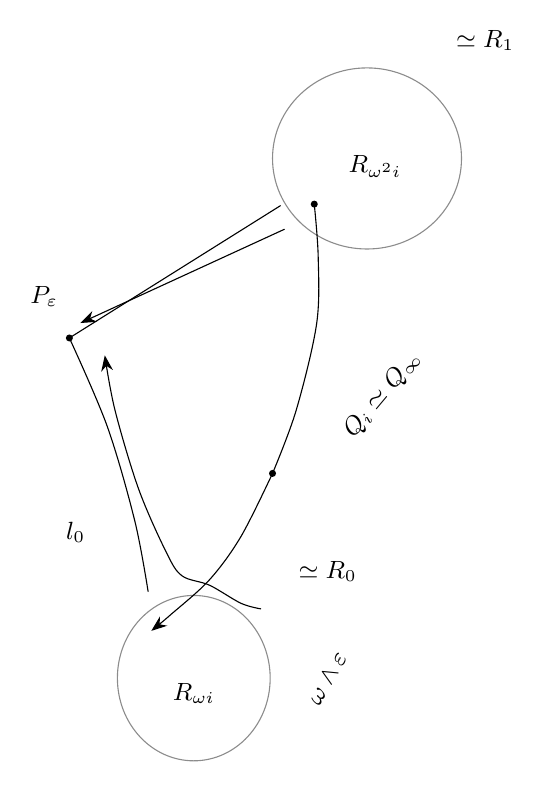
\begin{tikzpicture}[x=1mm,y=1mm,line cap=round,line join=round,font=\scriptsize]
\draw[pencil] (62,-26) ellipse[x radius=12, y radius=11.5];
\draw[pencil] (40,-92) ellipse[x radius=9.7, y radius=10.5];
\node[pt] at (24.2,-48.8) {};
\node[pt] at (55.3,-31.8) {};
\node[pt] at (50,-66) {};
\draw (24.2,-48.8) -- (51,-32);
\draw[-{Stealth[length=2mm]}] (51.5,-35) -- (25.6,-46.9);
\draw plot[smooth, tension=0.55] coordinates {(55.3,-31.8) (55.8,-38.5) (55.6,-47) (53,-58) (50,-66)};
\draw[-{Stealth[length=2mm]}] plot[smooth, tension=0.55] coordinates {(50,-66) (46,-74) (42,-79.5) (37,-84) (34.6,-86)};
\draw plot[smooth, tension=0.55] coordinates {(24.2,-48.8) (29,-60) (32.5,-72) (34.2,-81)};
\draw[-{Stealth[length=2mm]}] plot[smooth, tension=0.55] coordinates {(48.5,-83.2) (46,-82.5) (42,-80.2) (38.5,-79) (36.5,-76) (33,-68) (30,-58) (28.7,-51)};
\node[inner sep=1pt] at (21,-43.5) {\small $P_\varepsilon$};
\node[inner sep=1pt] at (63,-27) {\small $R_{\omega^2 i}$};
\node[inner sep=1pt] at (77,-11) {\small $\simeq R_1$};
\node[inner sep=1pt,rotate=50] at (64,-56) {\small $Q_{i}\simeq Q_\infty$};
\node[inner sep=1pt] at (25,-73.5) {\small $l_0$};
\node[inner sep=1pt] at (40,-94) {\small $R_{\omega i}$};
\node[inner sep=1pt] at (57,-78.5) {\small $\simeq R_0$};
\node[inner sep=1pt,rotate=60] at (57,-92) {\small $\omega\wedge\varepsilon$};
\end{tikzpicture}
\end{document}
